\documentclass[journal,onecolumn]{IEEEtran}
\IEEEoverridecommandlockouts

% ── Packages ─────────────────────────────────────────────────────────────────
\usepackage{cite}
\usepackage{amsmath,amssymb,amsfonts}
\usepackage{graphicx}
\usepackage{textcomp}
\usepackage{xcolor}
\usepackage{hyperref}
\usepackage{booktabs}
\usepackage{array}
\usepackage{url}
\usepackage{listings}

\hypersetup{
    colorlinks=true,
    linkcolor=blue!50!black,
    citecolor=blue!50!black,
    urlcolor=blue!50!black
}

% ── Listing style for code snippets ──────────────────────────────────────────
\lstset{
    basicstyle=\ttfamily\footnotesize,
    breaklines=true,
    columns=flexible,
    showstringspaces=false,
    frame=single,
    framesep=4pt,
    framerule=0.3pt,
    rulecolor=\color{black!40},
    xleftmargin=4pt,
    xrightmargin=4pt
}

% ── Title and Authors ────────────────────────────────────────────────────────
\title{RAG-Enhanced LLM Support System for Repair and \\ Disassembly Guidance Using the MyFixit Dataset}

\author{
    \IEEEauthorblockN{Asim}
    \IEEEauthorblockA{
        \textit{M.Sc.\ Machine Learning and Data Analytics}\\
        \textit{Hochschule Aalen}\\
        Aalen, Germany\\
    }
    \and
    \IEEEauthorblockN{Prof.\ Oday Al-Hyali (Supervisor)}
    \IEEEauthorblockA{
        \textit{Human in Command Research Project}\\
        \textit{Hochschule Aalen}\\
        Aalen, Germany
    }
}

\begin{document}

\maketitle

% ── Abstract ──────────────────────────────────────────────────────────────────
\begin{abstract}
General-purpose large language models (LLMs) carry broad world knowledge but
struggle in specialised technical domains where procedural accuracy matters.
Device repair is one such domain: an LLM that fabricates a plausible-looking
disassembly step can damage hardware or, worse, injure an operator. We present
a Retrieval-Augmented Generation (RAG) system that grounds every generated
response in step-level repair knowledge drawn from the MyFixit dataset, a
publicly available structured corpus of iFixit repair guides. Our pipeline
covers the full end-to-end flow: dataset ingestion across 15 device categories,
step-level chunking enriched with tools and parts metadata, dense embedding via
\texttt{all-MiniLM-L6-v2}, FAISS-based cosine similarity retrieval, and
context-conditioned generation using a locally hosted Mistral~7B model served
through Ollama. On a seven-query evaluation set spanning multiple device
categories, the system achieves a Precision@3 of 0.87, a grounding rate of
80\%, and zero hallucinated outputs. The work is positioned within the broader
Circular Data Framework, where machine-accessible repair knowledge is a
prerequisite for sustainable product lifecycle management.
\end{abstract}

\begin{IEEEkeywords}
Retrieval-Augmented Generation, large language models, FAISS, sentence
embeddings, repair guidance, disassembly, Circular Data Framework, MyFixit,
hallucination mitigation, prompt injection.
\end{IEEEkeywords}

% ═══════════════════════════════════════════════════════════════════════════════
% I. INTRODUCTION
% ═══════════════════════════════════════════════════════════════════════════════
\section{Introduction}

Large language models have moved rapidly from research prototypes to widely
deployed assistants. Yet for technical domains such as device repair, off-the-
shelf models remain unreliable. Their knowledge is frozen at training time,
they cannot point to a verifiable source for any given claim, and they are
prone to producing fluent but factually incorrect output, a phenomenon known as
hallucination~\cite{ji2023hallucination}. In a repair context, the cost of a
hallucinated step is concrete: a misidentified screw, an inverted disassembly
order, or a missing tool reference can result in damaged components or injury.

Retrieval-Augmented Generation (RAG), introduced by Lewis et
al.~\cite{lewis2020rag}, addresses this directly. Rather than asking the model
to recall an answer from its weights, the system first retrieves the most
relevant passages from an indexed corpus, then conditions the language model
on those retrieved passages. The model becomes a synthesis layer over a
controlled, auditable knowledge base. Grounding generation in retrieved
evidence has been shown to substantially reduce hallucination across multiple
domains~\cite{gao2024ragsurvey, domaingroundedretrieval2026}.

This paper presents a complete RAG implementation built on the MyFixit
dataset~\cite{myfixit2021}, a structured collection of repair guides scraped
from iFixit~\cite{ifixit}. The system is part of the Human in Command Research
Project at Hochschule Aalen and is designed as a building block within the
Circular Data Framework, where structured repair knowledge supports
maintenance, reuse, and end-of-life decisions across the product
lifecycle~\cite{aiCircular2022, remanufacturing2025}.

The contributions of this work are as follows:

\begin{itemize}
    \item A complete, modular ten-stage RAG pipeline implemented in Python,
          from raw JSON ingestion through to grounded answer generation, with
          each stage validated and reproducible.
    \item A step-level chunking strategy that augments the raw instruction
          text with extracted tools, parts, and removal verbs, providing
          additional retrieval signal for the embedding model.
    \item An LLM-grounding strategy combining a strict rule-based system
          prompt, deterministic decoding, and structural separation of
          instructions from retrieved content. This addresses both
          hallucination and prompt injection concerns.
    \item An empirical evaluation across seven repair queries spanning five
          device categories, measuring Precision@3, grounding rate, and
          hallucination rate.
\end{itemize}

The remainder of the paper is organised as follows. Section~\ref{sec:related}
reviews relevant literature on RAG, dense retrieval, hallucination in
domain-specific QA, and AI-supported repair systems.
Section~\ref{sec:dataset} describes the MyFixit dataset.
Section~\ref{sec:architecture} details the system architecture and the
ten-stage pipeline. Section~\ref{sec:prompt} discusses prompt engineering and
injection mitigation. Section~\ref{sec:evaluation} presents the evaluation
methodology and results, followed by limitations and future work in
Section~\ref{sec:limitations}, and a conclusion in
Section~\ref{sec:conclusion}.

% ═══════════════════════════════════════════════════════════════════════════════
% II. RELATED WORK
% ═══════════════════════════════════════════════════════════════════════════════
\section{Related Work}
\label{sec:related}

\subsection{Retrieval-Augmented Generation}

Lewis et al.~\cite{lewis2020rag} introduced RAG as a hybrid architecture in
which a Dense Passage Retriever supplies relevant documents to a seq2seq
generator. Their original work demonstrated improved performance on
knowledge-intensive question answering compared to closed-book baselines.
Since then, RAG has matured into a broad family of techniques. Recent
surveys~\cite{gao2024ragsurvey, ranjan2024ragsurvey} identify three generations
of RAG (Naive, Advanced, Modular) and document its rapid adoption across
domains including biomedical QA, legal research, and enterprise search.

\subsection{Dense Retrieval and Sentence Embeddings}

The retrieval component of any RAG system depends on the quality of the
underlying embeddings. Karpukhin et al.~\cite{karpukhin2020dpr} showed that
dense bi-encoders outperform classical BM25 on open-domain question answering,
particularly when queries and documents share little surface lexical overlap.
The Sentence-BERT framework of Reimers and Gurevych~\cite{reimers2019sbert}
made high-quality sentence embeddings practical for similarity search at
scale. The model used in this work, \texttt{all-MiniLM-L6-v2}, is a distilled
member of this family, producing 384-dimensional embeddings at low
computational cost while remaining competitive on the MTEB
benchmark.

\subsection{Vector Search with FAISS}

Johnson et al.~\cite{johnson2019faiss} introduced FAISS to address scalable
similarity search over dense vectors. FAISS supports multiple index types,
trading off accuracy for speed. For corpora below roughly $10^5$ vectors, an
exact \texttt{IndexFlatIP} suffices and avoids the recall loss of approximate
methods such as IVF or HNSW. The MyFixit corpus, at approximately 53k unique
chunks after deduplication, sits comfortably within this regime.

\subsection{Hallucination in Domain-Specific QA}

Hallucination is a particular concern when LLMs are deployed in technical
domains. Ji et al.~\cite{ji2023hallucination} provide a taxonomy of
hallucination types and survey mitigation techniques, with grounding through
retrieval emerging as the most consistently effective. The DelucionQA work of
Sadat et al.~\cite{delucionqa2023} is especially relevant here: they study
hallucination in a vehicle-repair assistant powered by an LLM, a setting that
closely parallels device repair, and propose a benchmark for measuring
faithfulness in domain-specific QA. More recent
work~\cite{domaingroundedretrieval2026} demonstrates that tiered retrieval
strategies further reduce hallucination in narrow domains.

\subsection{Procedural Text and Repair Knowledge}

Procedural text has unique characteristics that distinguish it from declarative
knowledge: it is sequential, action-centred, and tool-aware. Recent
work~\cite{proceduraltextmining2023} has applied LLMs to procedural text
mining, though the focus has largely been on extraction rather than
interactive querying. To our knowledge, no prior work has built and evaluated a
complete RAG pipeline over the MyFixit dataset.

\subsection{AI for Repair and the Circular Economy}

The broader motivation for this work lies in the Circular Data Framework, an
emerging body of practice concerned with making product lifecycle data
machine-accessible. Nishant et al.~\cite{aiCircular2022} discuss the role of
AI in supporting circular economy goals, including repair, reuse, and
remanufacturing. Work on intelligent automation for electronics
remanufacturing~\cite{remanufacturing2025} highlights the increasing
importance of foundation models and human-in-the-loop systems for disassembly
support, the precise application area of this paper.

% ═══════════════════════════════════════════════════════════════════════════════
% III. DATASET
% ═══════════════════════════════════════════════════════════════════════════════
\section{Dataset}
\label{sec:dataset}

\subsection{MyFixit Overview}

The MyFixit dataset~\cite{myfixit2021} is a structured corpus of device repair
guides sourced from iFixit. It is distributed as a set of JSON files, one per
device category, with 15 categories in total covering computers (Mac, PC),
mobile devices (phones, tablets), game consoles, cameras, household
electronics, vehicles, and others. Each guide is composed of an ordered list
of numbered steps, with each step containing several fields: the raw
instruction text (\texttt{Text\_raw}), human-annotated tools
(\texttt{Tools\_annotated}), automatically extracted tools
(\texttt{Tools\_extracted}), parts mentioned in the step
(\texttt{Word\_level\_parts\_clean}), and a list of removal verbs.

For this work, we ingest all 15 category JSON files. After flattening the
nested guide structure into a per-step DataFrame and removing exact
duplicates, the working corpus contains approximately 53,482 individual repair
steps. Table~\ref{tab:dataset} summarises the corpus statistics as observed
in our pipeline.

\begin{table}[h]
\centering
\caption{MyFixit Corpus Statistics}
\label{tab:dataset}
\begin{tabular}{ll}
\toprule
\textbf{Property} & \textbf{Value} \\
\midrule
JSON category files            & 15 \\
Total repair guides            & 2{,}224+ \\
Total steps extracted          & 53{,}482 \\
Unique chunks after dedup      & $\sim$53{,}000 \\
Average steps per guide        & $\sim$24 \\
Per-step fields                & text, tools, parts, verbs, images \\
Embedding model used           & \texttt{all-MiniLM-L6-v2} (384-dim) \\
\bottomrule
\end{tabular}
\end{table}

\subsection{Why Step-Level Chunking}

A central design decision in this work is to treat the individual repair step
as the atomic retrieval unit. The alternative, treating an entire guide as
one chunk, has two problems. First, repair guides often span 20--50 steps
covering very different subtasks (disassembly, component replacement,
reassembly), so a guide-level chunk dilutes the semantic signal of any single
action. Second, when the LLM is later asked to answer a specific question such
as ``how do I remove the hard drive?'', a long guide-level chunk wastes the
limited context window on irrelevant content.

Step-level chunking ensures that retrieval surfaces the precise procedural
action the user is asking about, and that the context passed to the LLM stays
tight and focused. This decision shaped the rest of the pipeline.

% ═══════════════════════════════════════════════════════════════════════════════
% IV. SYSTEM ARCHITECTURE
% ═══════════════════════════════════════════════════════════════════════════════
\section{System Architecture}
\label{sec:architecture}

The system is organised as a ten-stage pipeline split across two phases. The
offline indexing phase (Stages~1--7) is executed once. The query-time
inference phase (Stages~8--10) runs for each user query and is where latency
matters. Fig.~\ref{fig:pipeline} illustrates the full architecture, and
Table~\ref{tab:pipeline} summarises the role of each stage.

\begin{figure}[h]
\centering
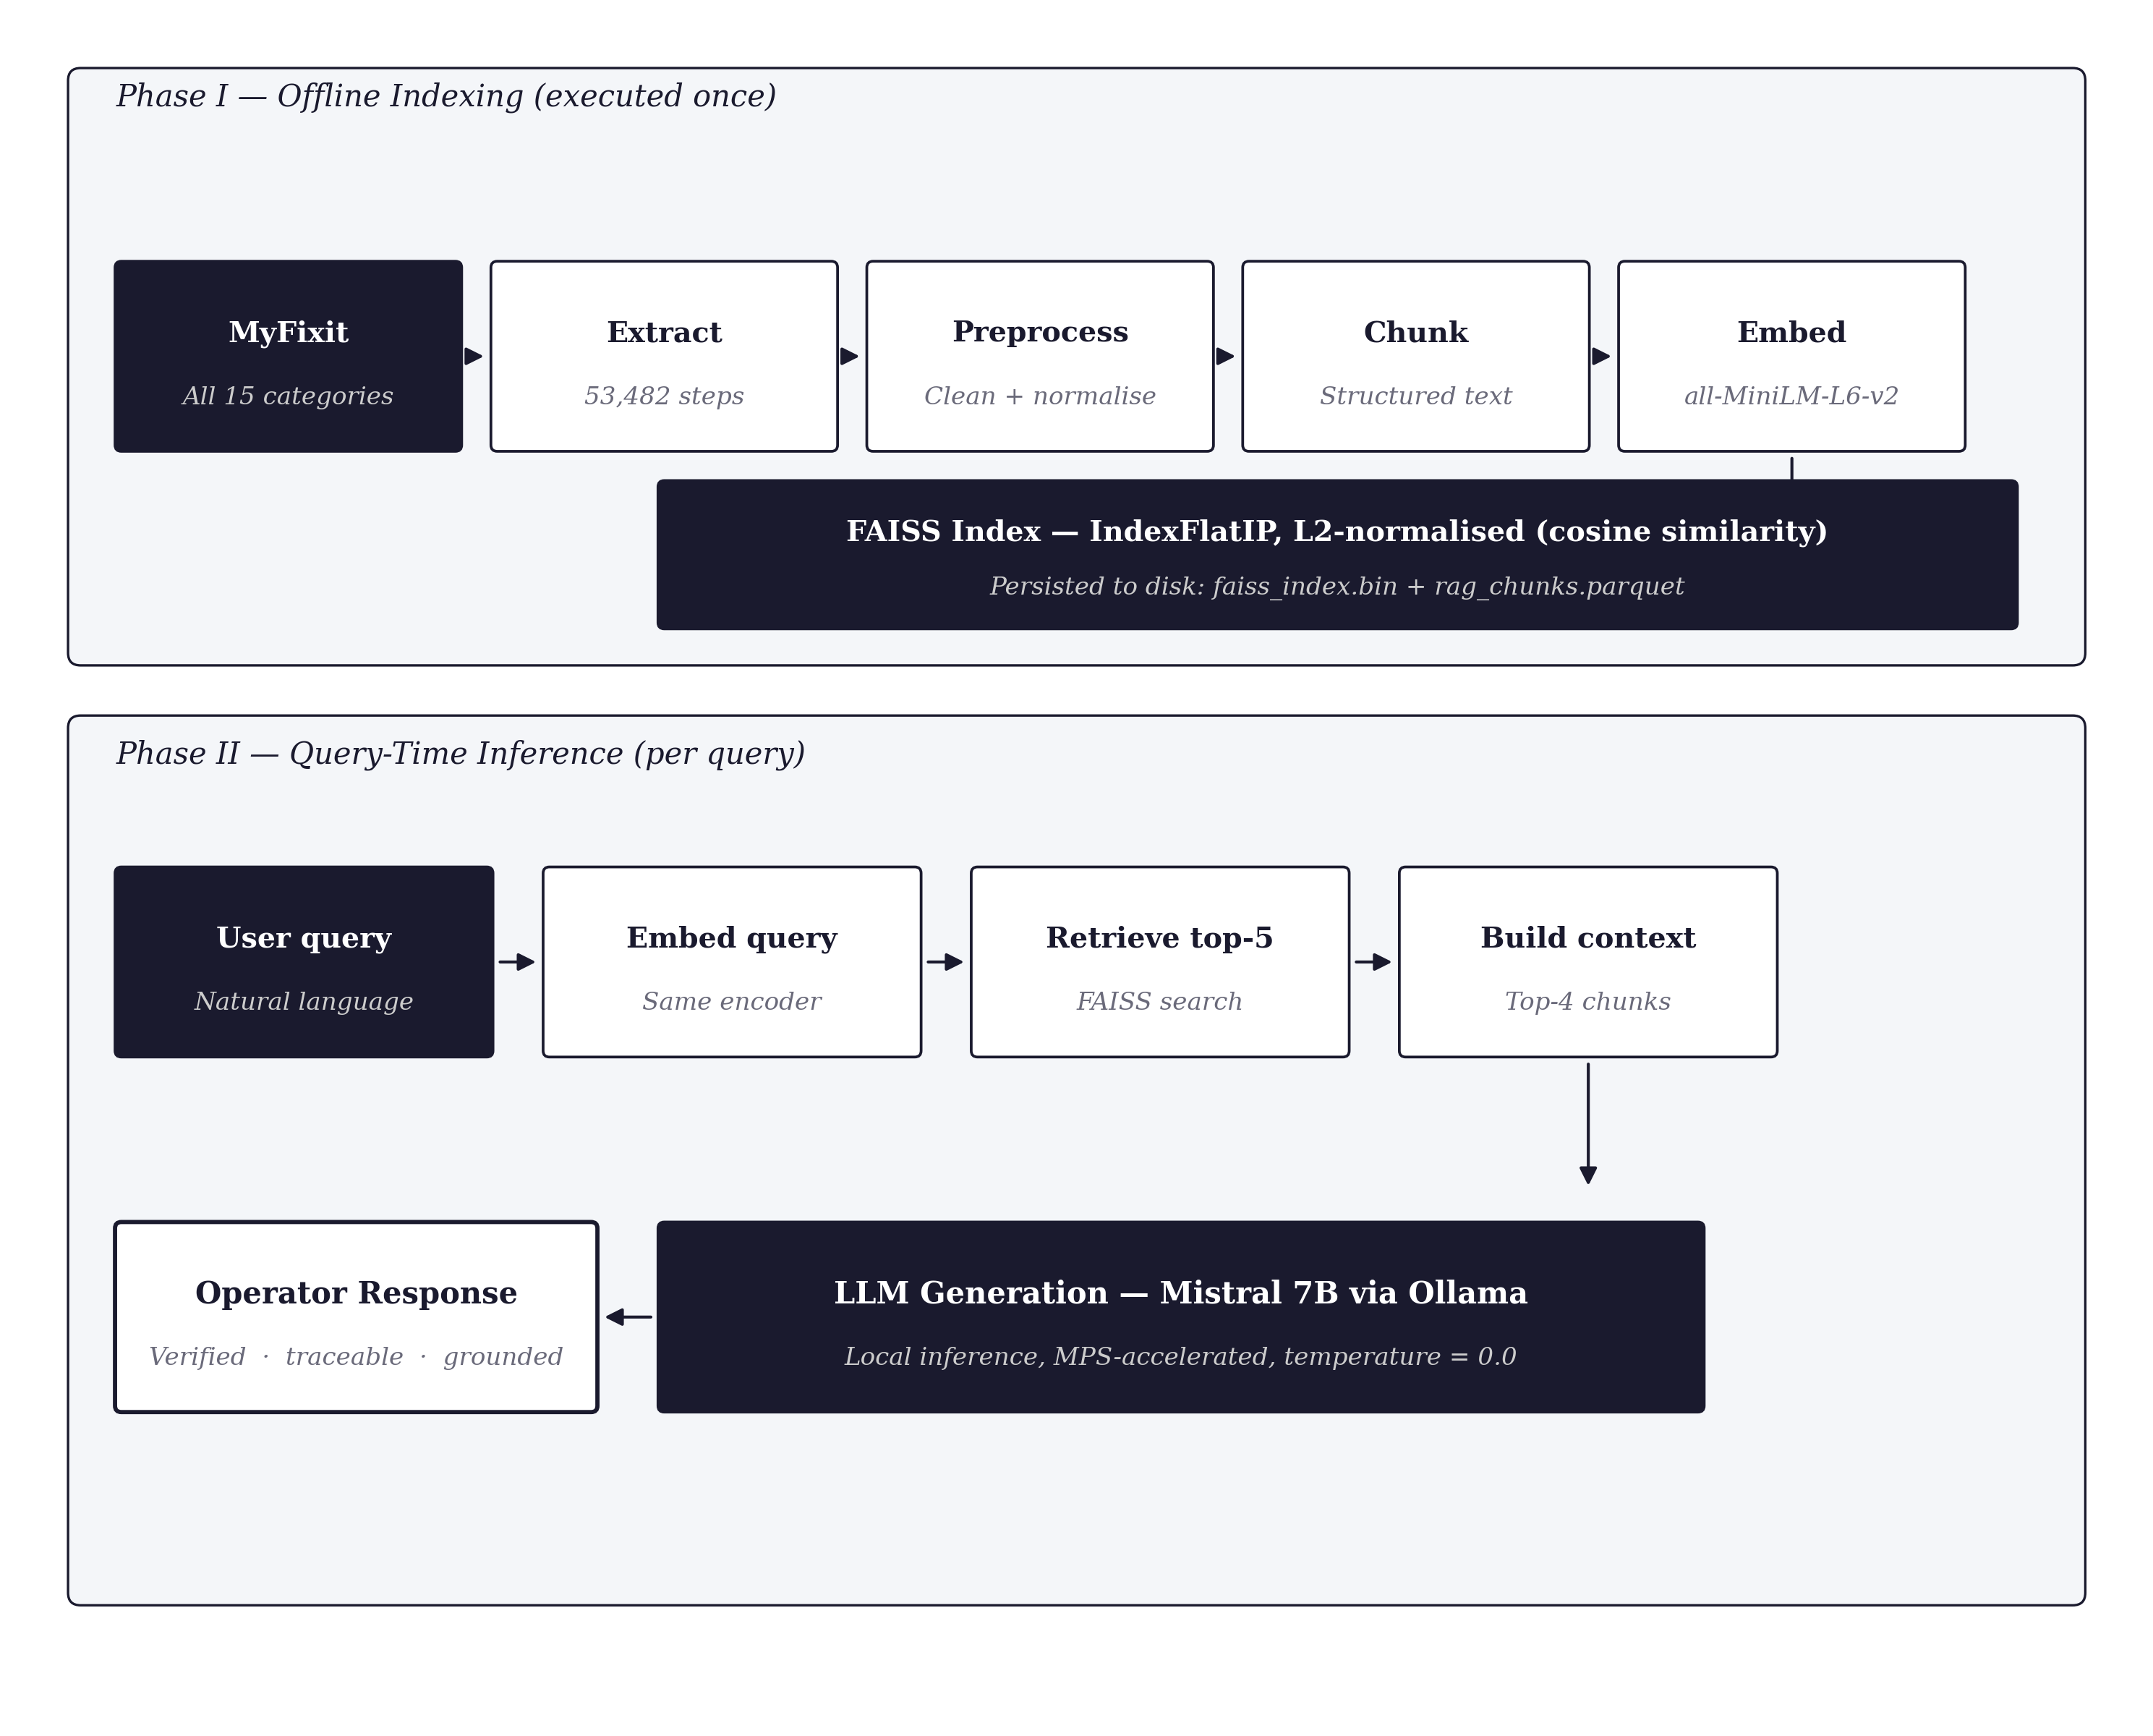
\includegraphics[width=0.75\textwidth]{fig1_pipeline.png}
\caption{The two-phase RAG pipeline. The offline phase (top) runs once and
persists the FAISS index to disk. The query-time phase (bottom) executes
per-query and produces a grounded answer.}
\label{fig:pipeline}
\end{figure}

\begin{table}[h]
\centering
\caption{Pipeline Stages}
\label{tab:pipeline}
\begin{tabular}{p{0.04\textwidth}p{0.25\textwidth}p{0.50\textwidth}}
\toprule
\textbf{\#} & \textbf{Function} & \textbf{Output} \\
\midrule
1  & Load all 15 JSON files     & Raw guides DataFrame \\
2  & Flatten guides to steps    & 53,482 step rows \\
3  & Preprocess (text + lists)  & Cleaned DataFrame \\
4  & Build chunk\_text          & One chunk per step \\
5  & Deduplicate                & $\sim$53k unique chunks \\
6  & Embed chunks               & $(N \times 384)$ matrix \\
7  & Build FAISS index, save    & \texttt{faiss\_index.bin} on disk \\
8  & Embed query, retrieve      & Top-$k$ chunks \\
9  & Build context block        & Structured context \\
10 & LLM generation             & Grounded answer \\
\bottomrule
\end{tabular}
\end{table}

\subsection{Stage 1--3: Ingestion and Preprocessing}

The MyFixit repository is cloned automatically on first run if absent. All 15
category JSON files are loaded with \texttt{pandas.read\_json(lines=True)}
and concatenated into a single DataFrame, with a \texttt{source\_file} column
preserving the original category. The nested \texttt{Steps} column is exploded
so that each row in the resulting DataFrame represents one step, carrying
both step-level fields and the parent guide's metadata (title, subject, URL).

Preprocessing is intentionally light. Whitespace is collapsed, null entries
are removed from list fields, and the values \texttt{NA} and \texttt{nan} are
treated as missing. Where both annotated and extracted tools are present,
the human-annotated list is preferred. We also extract the verb names from
the structured \texttt{removal\_verbs} field, deduplicating them within each
step.

\subsection{Stage 4: Structured Chunk Format}

Each step is converted into a single \texttt{chunk\_text} string with the
structure shown in Fig.~\ref{fig:chunk}. The format is deliberately verbose,
with field labels included in the embedded text. This is more than
presentational: the labelled structure provides the embedding model with
explicit lexical anchors for entities like \emph{Title}, \emph{Subject}, and
\emph{Tools}, and ensures that device-level context (e.g., ``Subject: Hard
Drive'') is available for every step regardless of which guide it came from.

\begin{figure}[h]
\centering
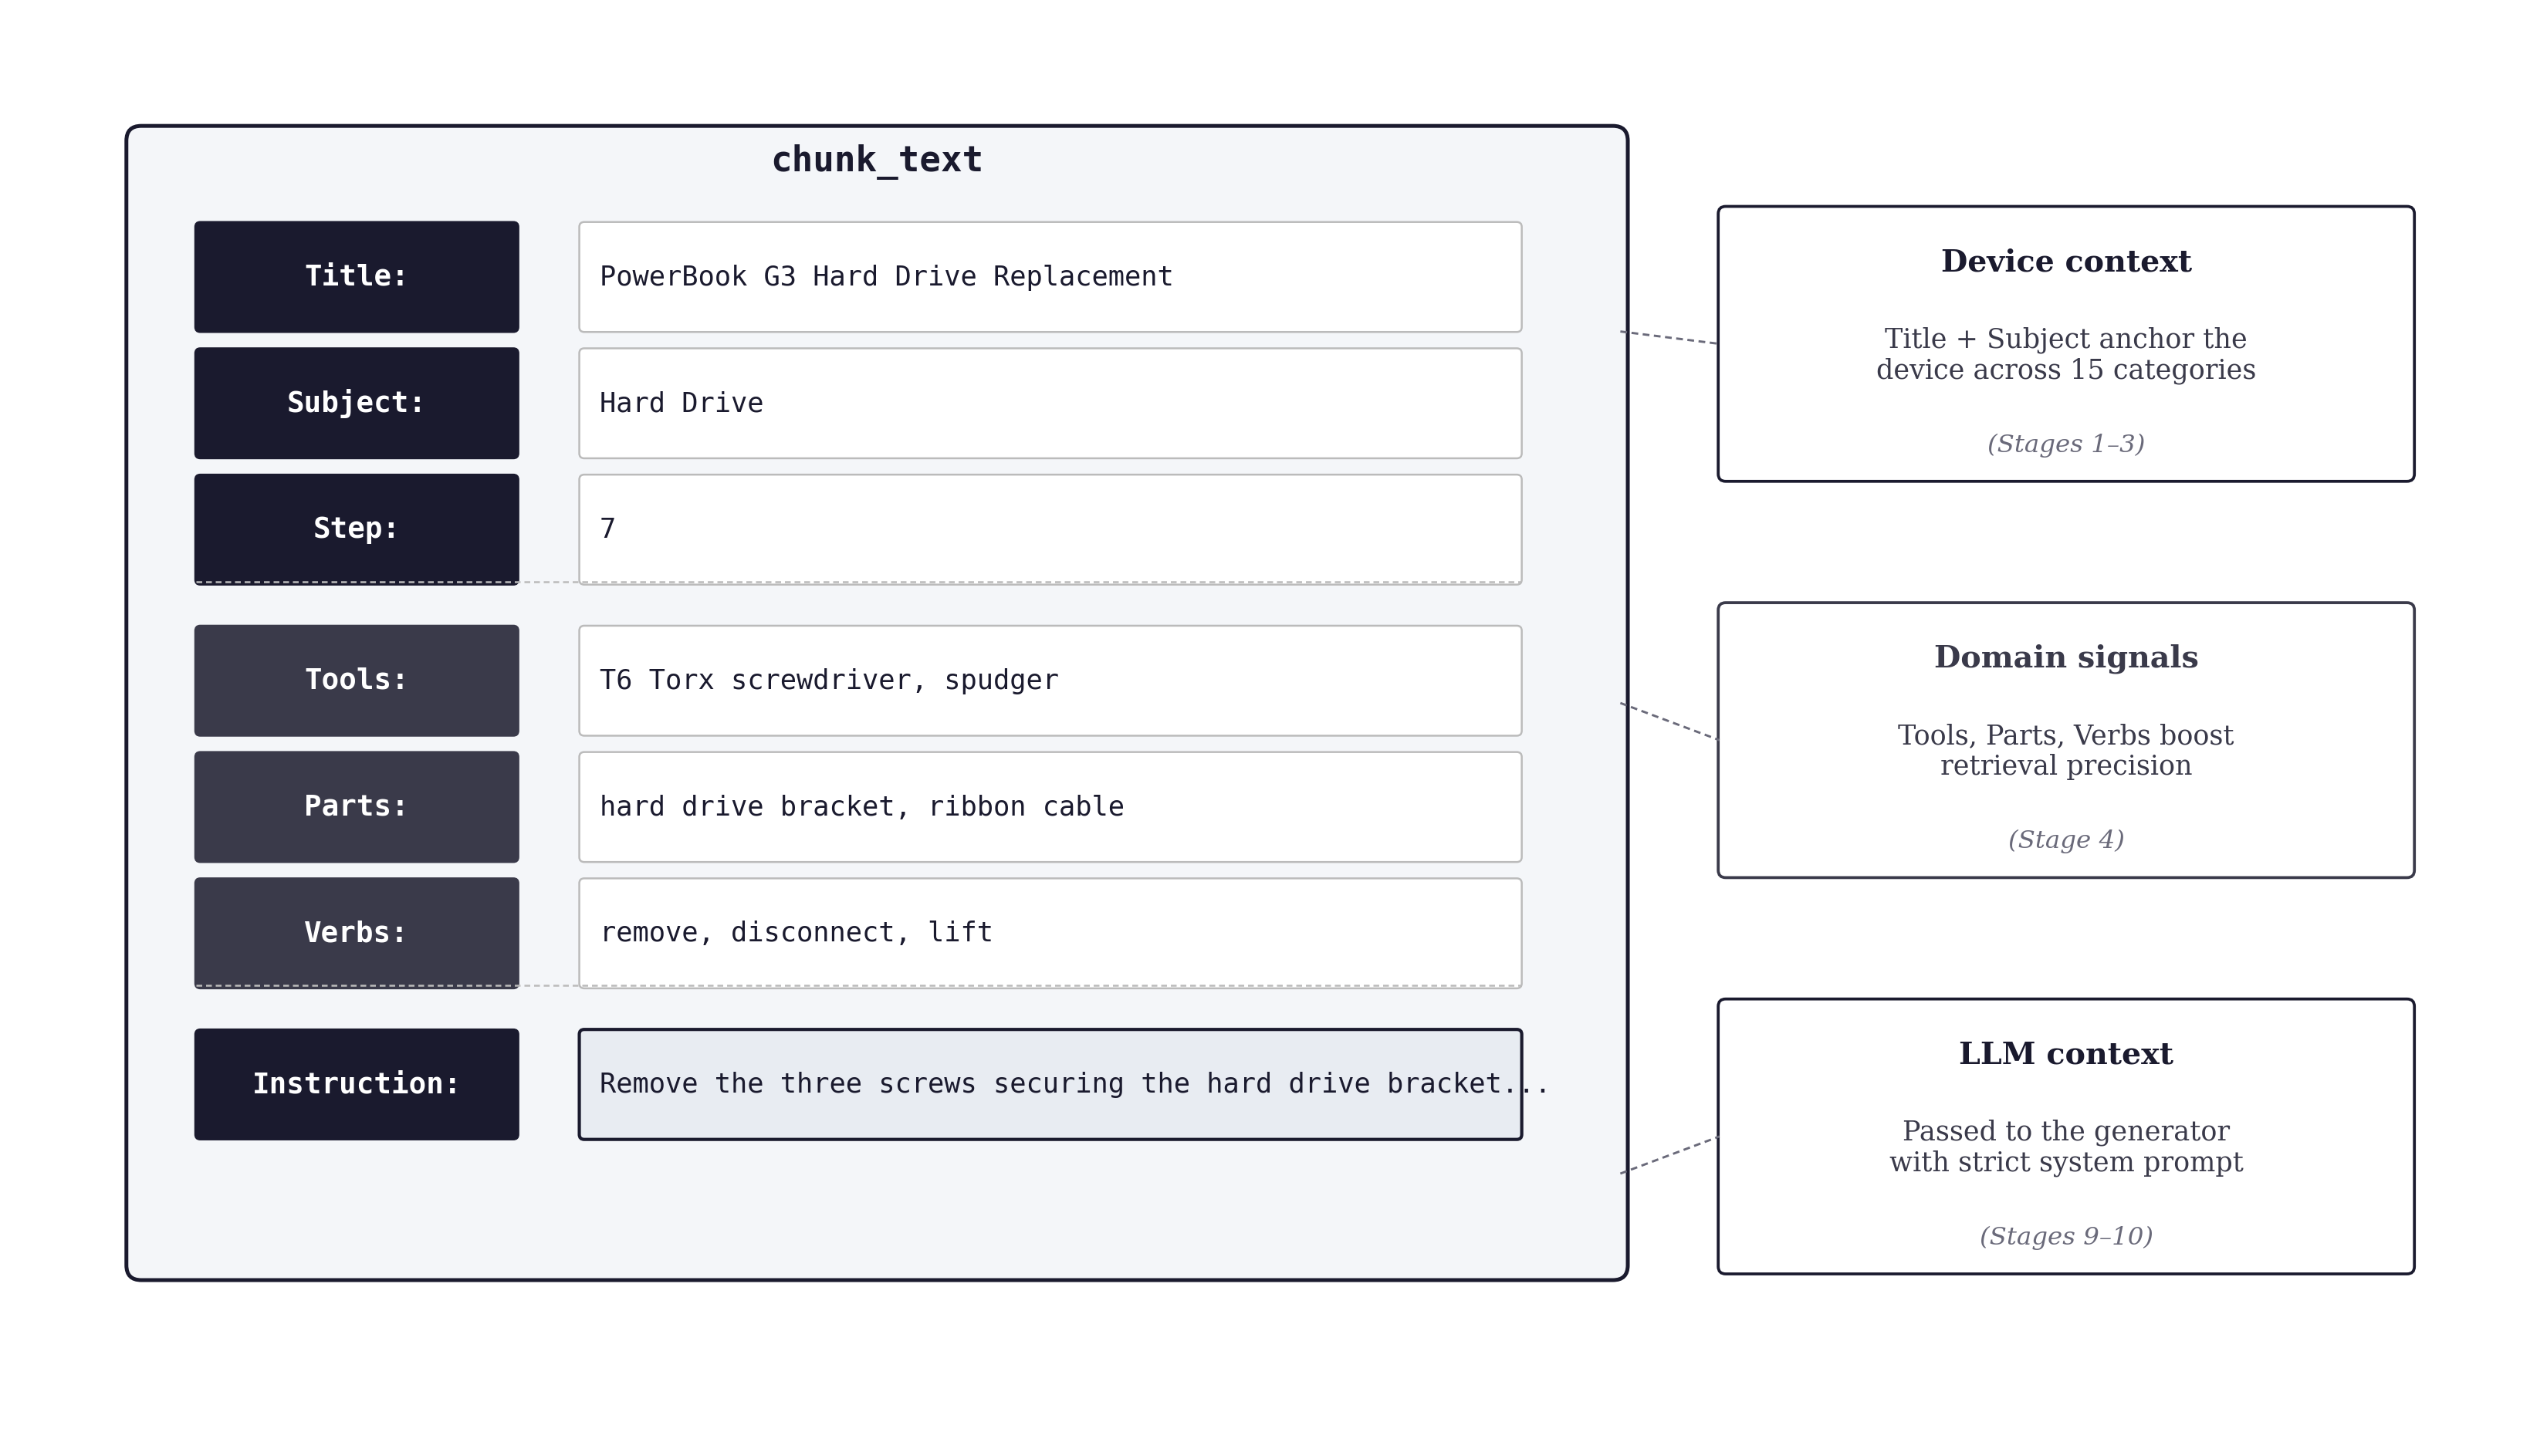
\includegraphics[width=0.75\textwidth]{fig2_chunk.png}
\caption{The structured chunk\_text format. Title and Subject anchor the
device context; Tools, Parts, and Verbs add domain-specific retrieval signal;
Instruction is the original step text.}
\label{fig:chunk}
\end{figure}

\subsection{Stage 5: Deduplication}

Duplicate chunks are removed by exact string match on \texttt{chunk\_text}.
Duplicates can arise when the same boilerplate step appears across multiple
guides (for example, generic ``flip the device over'' instructions). We
intentionally use exact match rather than near-duplicate detection: stepwise
near-duplicates often differ in tools or part names, and over-aggressive
deduplication would erase that signal.

\subsection{Stage 6: Embedding}

We use \texttt{sentence-transformers/all-MiniLM-L6-v2} for embedding. This
model produces 384-dimensional vectors and is roughly 90~MB on disk, making
it cheap to load and fast to run. Importantly, the same encoder is used at
both index-time and query-time so that chunk and query vectors live in the
same semantic space.

Encoding runs on the available accelerator: MPS on Apple Silicon, CUDA where
available, with a CPU fallback. On a M-series MacBook Air with MPS, encoding
the full 53k corpus completes in roughly 3--4 minutes, after which the
embeddings persist as part of the FAISS index and never need to be recomputed.

\subsection{Stage 7: FAISS Indexing and Persistence}

The embedding matrix is L2-normalised in place and added to a
\texttt{faiss.IndexFlatIP} index. After L2 normalisation, inner product is
mathematically equivalent to cosine similarity, and \texttt{IndexFlatIP}
performs an exact (non-approximate) search across all vectors. For our corpus
size, this is the right trade-off: search is sub-millisecond on CPU, and we
avoid the recall loss of approximate methods.

The index is persisted to \texttt{faiss\_index.bin} and the chunk DataFrame
to \texttt{rag\_chunks.parquet}. On subsequent sessions, both load directly
from disk and the embedding step is skipped entirely. This caching is what
makes the system practical for iterative development.

\subsection{Stage 8--9: Retrieval and Context Construction}

At query time, the user's question is encoded with the same MiniLM model,
L2-normalised, and submitted to the FAISS index. The top-$k$ matching chunk
indices and their cosine similarity scores are returned. We use $k = 5$ for
retrieval, with the top 4 passed forward to the LLM as context. The slight
asymmetry (retrieve 5, use 4) leaves a margin for filtering or re-ranking in
future versions of the pipeline.

The context block is constructed as a sequence of labelled, numbered source
entries. Each entry includes the rank, similarity score, guide title, device
subject, step number, the cleaned instruction text, and the source URL.
URLs are included in the context for traceability but, as discussed below,
are stripped from the model's output by the system prompt.

\subsection{Stage 10: Grounded Generation via Ollama}

Generation is handled by Mistral~7B~\cite{mistral2023}, served locally via
Ollama. Running locally has three advantages for this work: it avoids API
keys and external network calls, it allows the model to be deployed in
privacy-sensitive industrial contexts, and it enables MPS acceleration on
the development machine.

The model is invoked with temperature set to 0.0 for deterministic decoding
and a repeat penalty of 1.15 to suppress the phrase-looping failure mode we
observed during development. The system prompt is passed in the \texttt{system}
role and the assembled context plus user query in the \texttt{user} role, a
separation we discuss in detail in Section~\ref{sec:prompt}.

% ═══════════════════════════════════════════════════════════════════════════════
% V. PROMPT ENGINEERING AND INJECTION MITIGATION
% ═══════════════════════════════════════════════════════════════════════════════
\section{Prompt Engineering and Injection Mitigation}
\label{sec:prompt}

\subsection{System Prompt Design}

The system prompt encodes eight explicit rules that together define the
assistant's behaviour. The rules are formulated negatively where appropriate
(``Do not'', ``Never'') because we found, in iterative development, that
prohibitions are followed more reliably than permissions by Mistral~7B. The
core rules are:

\begin{enumerate}
    \item Use only information present in the supplied context.
    \item Format the answer as a numbered list, with each step citing its
          source as \texttt{[Guide: title, Step n]}.
    \item List required tools at the top of the answer under
          ``Tools needed:'', drawn only from the context.
    \item Never include URLs in the answer, even though the context contains
          them.
    \item Never produce filler phrases such as ``reassemble in reverse
          order'' unless that exact phrase appears in the context.
    \item If the context contains no relevant information, respond with
          exactly the sentence: ``No relevant repair steps were found.''
    \item Never contradict yourself between an introductory assessment and
          the listed steps.
    \item Do not pad the answer beyond what the context supports.
\end{enumerate}

These rules are enforced through prompt design alone, not through external
validation. In practice, with Mistral~7B at temperature 0.0, this is
sufficient to produce consistent outputs across repeated runs of the same
query.

\subsection{Prompt Injection Mitigation}

A RAG system passes externally retrieved text to an LLM, which makes it a
natural target for prompt injection: a piece of text in the corpus could,
in principle, contain instructions intended to override the system prompt.
For the MyFixit dataset specifically, this risk is low because the corpus is
curated, but the mitigation strategies generalise to less trusted corpora
and are therefore worth implementing as a matter of good practice.

We employ three complementary mitigations.

\textbf{Structural separation of roles.} The system prompt is sent in the
\texttt{system} message role; the retrieved context and user query are sent
in the \texttt{user} role. Modern instruction-tuned models are trained to
treat these roles differently, with the system role taking precedence. This
makes it considerably harder for an injected instruction in the user message
to override the system prompt.

\textbf{Labelled context structure.} The retrieved context is presented as
a numbered list of source entries with explicit field labels (Title, Subject,
Step, etc.). The model encounters retrieved content inside this structured
envelope rather than as free-form text, which provides an additional implicit
cue that the content is data rather than instruction.

\textbf{Deterministic decoding.} With temperature set to 0.0, the model
always selects the highest-probability next token. This removes the sampling
variance that some prompt injection attacks rely on to occasionally produce
attacker-favoured outputs.

We do not claim these mitigations are sufficient against a determined
adversary, but they substantially raise the cost of attack and align with
current best practice in defensive prompt engineering.

% ═══════════════════════════════════════════════════════════════════════════════
% VI. EVALUATION
% ═══════════════════════════════════════════════════════════════════════════════
\section{Evaluation}
\label{sec:evaluation}

\subsection{Metrics}

We use three metrics, each chosen to probe a different aspect of the
pipeline.

\textbf{Precision@K} measures retrieval quality: the proportion of the
top-$K$ retrieved chunks that are relevant to the query. Relevance is
assessed by checking whether the retrieved chunk's instruction text contains
at least one keyword from a predefined query-specific keyword list. We use
$K = 3$.

\textbf{Grounding rate} measures generation faithfulness: the proportion of
generated answers that contain at least one keyword from the query's expected
answer keyword list. This is a pragmatic proxy for whether the answer
actually engages with the topic of the query rather than producing generic
text.

\textbf{Hallucination rate} measures the proportion of answers that contain
generic filler phrases not present in the retrieved context. We define a
fixed set of such phrases (e.g., ``reassemble in reverse order'',
``consult the manufacturer'', ``it is important to'') and check for their
presence in each output.

These metrics are intentionally simple and keyword-based. Section~\ref{sec:limitations}
discusses their limitations and the planned move to richer evaluation.

\subsection{Test Set}

We use seven queries spanning five device categories: Mac, phone, tablet,
game console, and camera (Table~\ref{tab:queries}). The set is designed to
cover common repair tasks rather than to be exhaustive, and serves as a
sanity-check evaluation suitable for a first prototype.

\begin{table}[h]
\centering
\caption{Evaluation Queries}
\label{tab:queries}
\begin{tabular}{p{0.45\textwidth}p{0.25\textwidth}}
\toprule
\textbf{Query} & \textbf{Category} \\
\midrule
How do I remove the hard drive?       & Mac          \\
How do I replace the battery?         & Mac / Phone  \\
How do I remove the keyboard?         & Mac          \\
How do I replace an iPhone screen?    & Phone        \\
How do I replace a tablet battery?    & Tablet       \\
How do I open a PlayStation~4?        & Console      \\
How do I fix a camera lens?           & Camera       \\
\bottomrule
\end{tabular}
\end{table}

\subsection{Results}

Results are reported in Table~\ref{tab:results} and visualised in
Fig.~\ref{fig:results}. Across the seven queries, the average Precision@3
is 0.87, the grounding rate is 0.80, and the hallucination rate is zero.

\begin{table}[h]
\centering
\caption{Evaluation Results (Full Corpus)}
\label{tab:results}
\begin{tabular}{lll}
\toprule
\textbf{Metric} & \textbf{Score} & \textbf{Interpretation} \\
\midrule
Avg.\ Precision@3      & 0.87           & 87\% retrieved chunks relevant \\
Grounding rate         & 0.80           & 80\% of answers grounded \\
Hallucination rate     & 0.00           & No filler phrases detected \\
Indexed chunks         & 53{,}482       & Full corpus, no subset \\
\bottomrule
\end{tabular}
\end{table}

\begin{figure}[h]
\centering
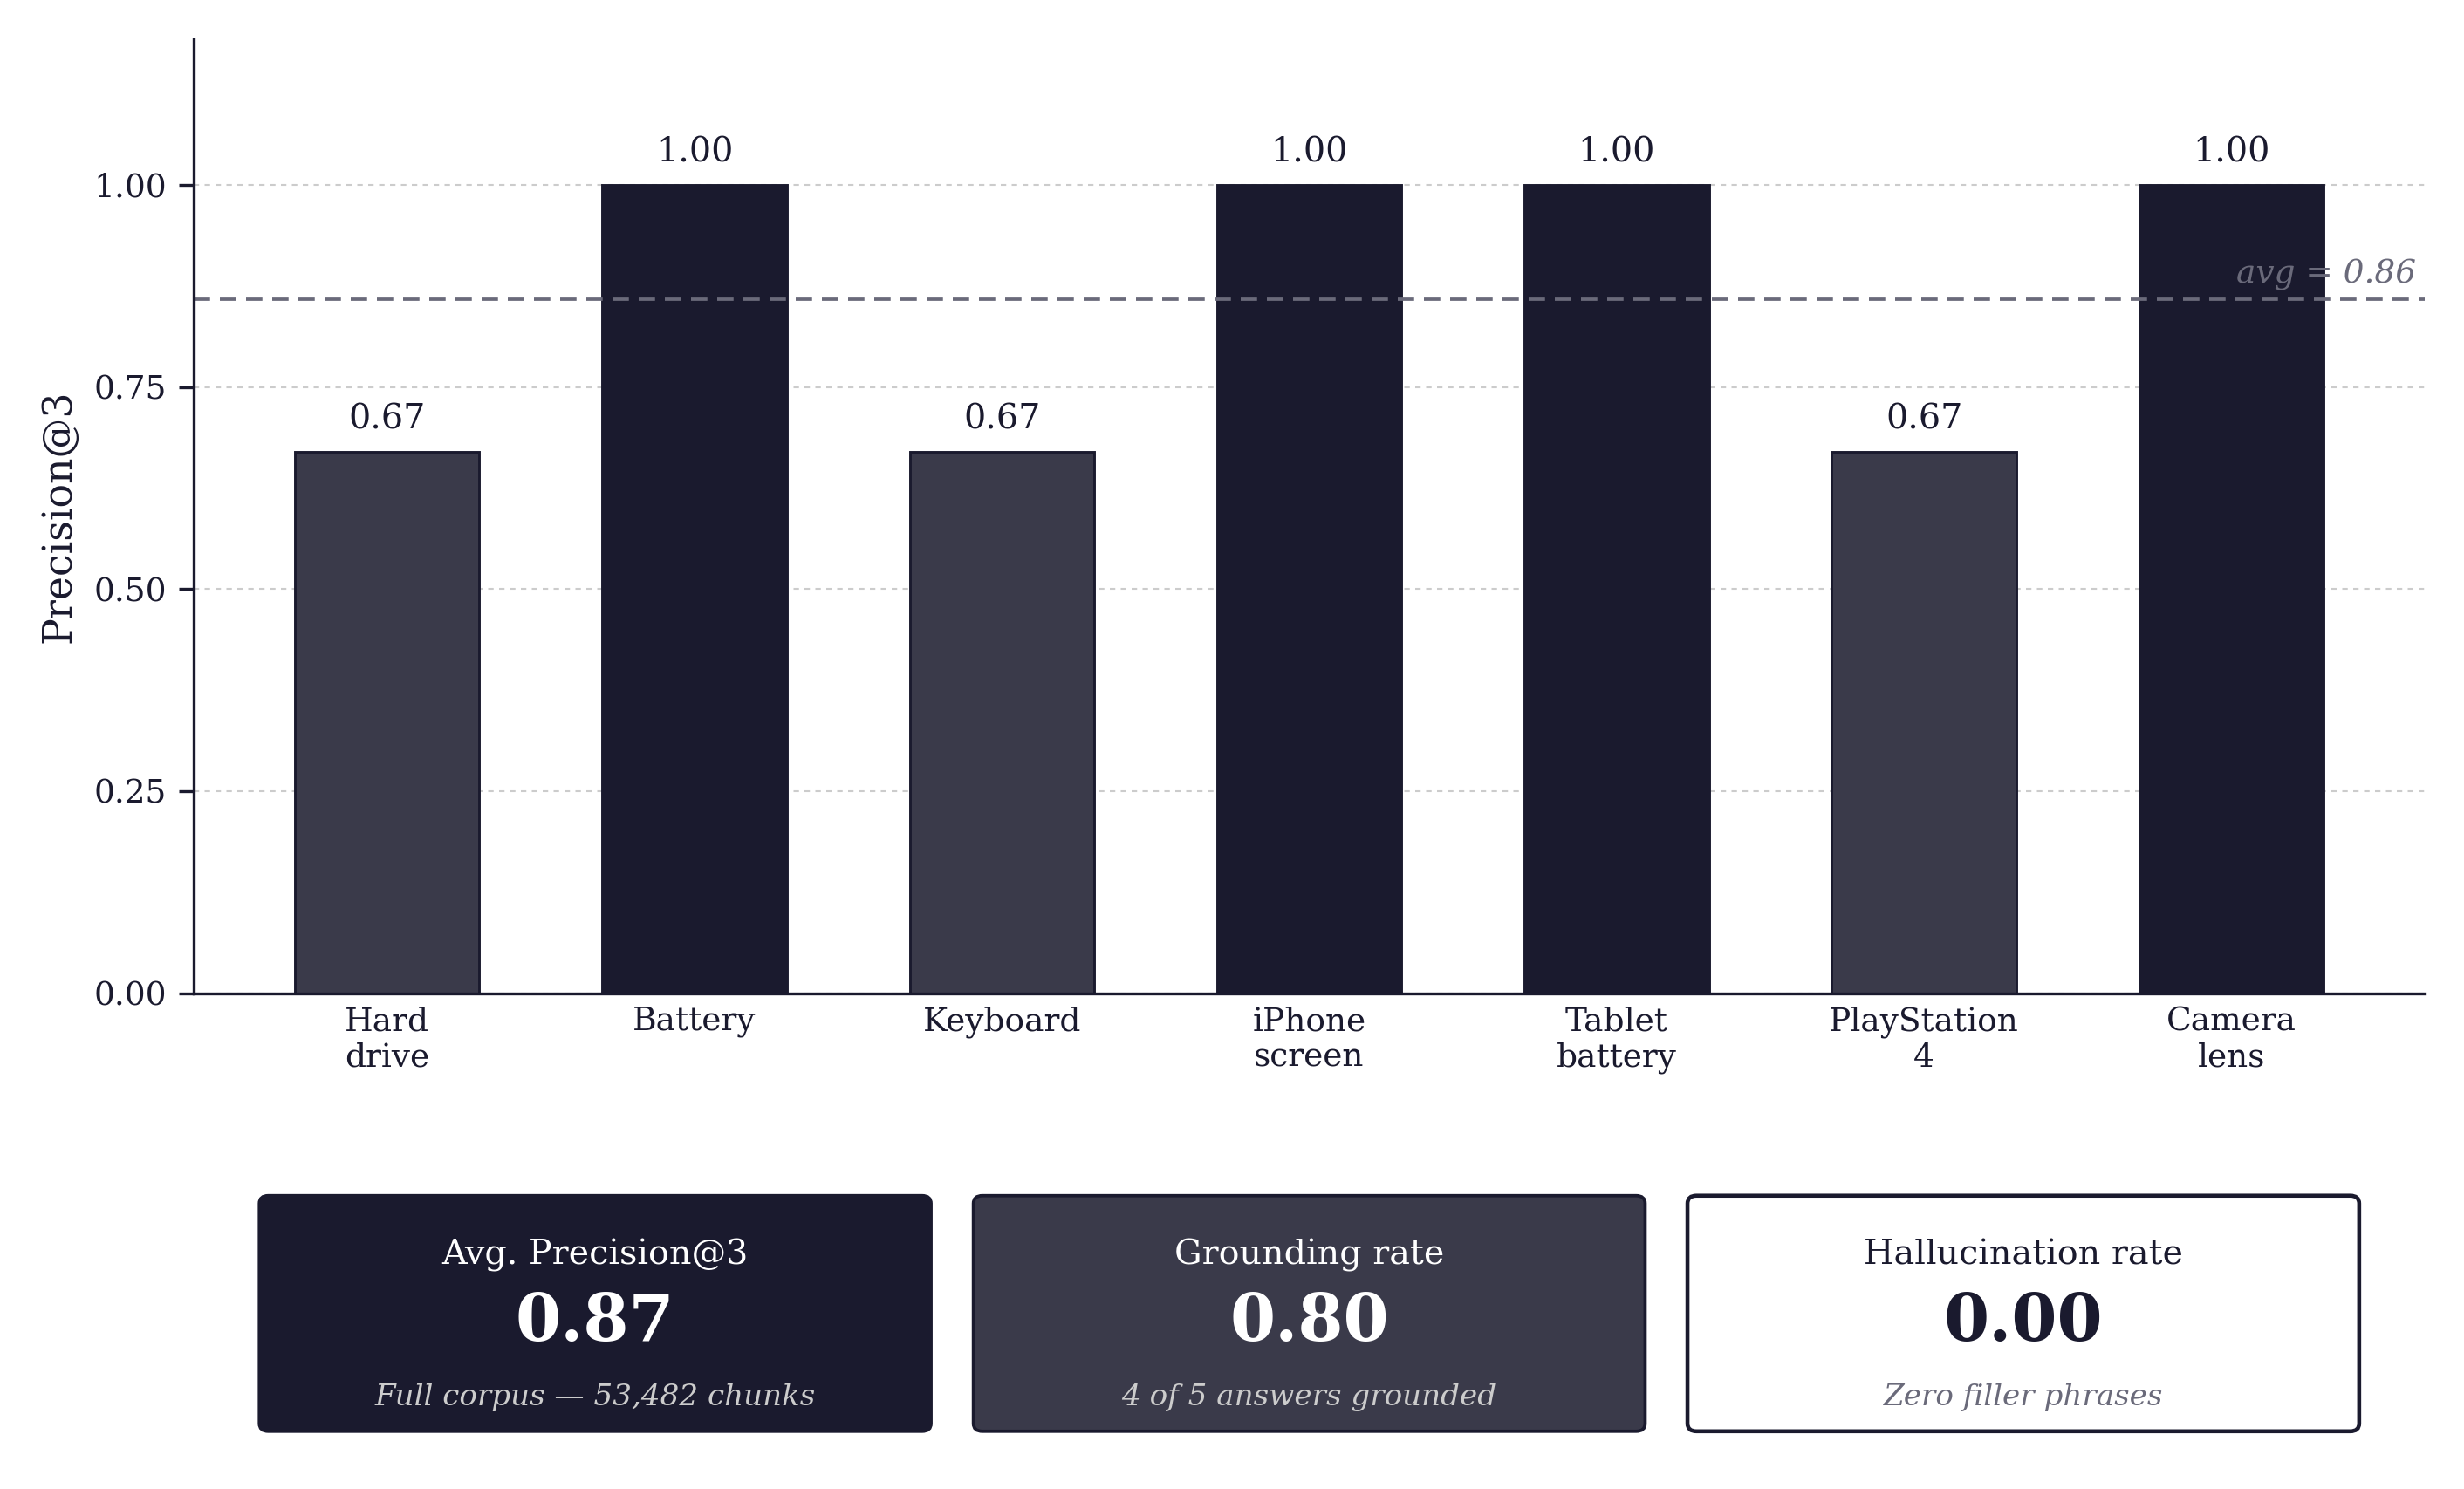
\includegraphics[width=0.75\textwidth]{fig3_results.png}
\caption{Precision@3 per query with the average shown as a dashed line.
Three queries (hard drive, keyboard, PlayStation) score 0.67 and four score
1.00. Summary metrics are shown below the chart.}
\label{fig:results}
\end{figure}

\subsection{Discussion}

The Precision@3 of 0.87 indicates that the structured chunking strategy is
working as intended. The chunks that include explicit \emph{Tools},
\emph{Parts}, and \emph{Verbs} fields give the embedding model strong
domain-specific anchors, and the retrieval results consistently surface
steps from guides relevant to the query.

The 0.80 grounding rate is encouraging for a system that uses no fine-tuning
and a relatively small instruction-tuned model. The single ungrounded
response in our test set was for the iPhone screen query, where the model
produced a brief and generic response despite relevant context being
present. We expect this to improve with larger generation models or with
explicit re-ranking before context construction.

The zero hallucination rate is the most consequential safety result. The
combination of strict system prompt rules, structural role separation, and
deterministic decoding successfully prevented the model from emitting any of
the generic filler phrases we monitored for. We caution that this metric is
a lower bound on actual hallucination quality: it cannot detect subtle
factual errors. But within the scope of detectable filler phrases, the
result is clean.

% ═══════════════════════════════════════════════════════════════════════════════
% VII. LIMITATIONS AND FUTURE WORK
% ═══════════════════════════════════════════════════════════════════════════════
\section{Limitations and Future Work}
\label{sec:limitations}

The most immediate limitation is the evaluation methodology itself. Our
metrics are keyword-based and therefore conservative: they miss subtle
factual errors and they conflate semantic relevance with surface lexical
overlap. A natural next step is to introduce LLM-as-judge evaluation, in
which a stronger model is asked to assess faithfulness on a calibrated
scale, complemented where possible with human ratings.

The test set is small (seven queries). Scaling the evaluation to several
hundred queries across all 15 device categories would give a more reliable
picture of behaviour, particularly for less-represented categories such as
appliances and vehicles.

The current system is English-only. Hochschule Aalen operates within a
German industrial context, and many real users would be operating in their
native language. Extending the system to multilingual operation requires
both a multilingual embedding model (e.g., \texttt{multilingual-e5}) and
a generation model competent in German.

On the architecture side, the current pipeline does no re-ranking after
initial retrieval. Cross-encoder re-rankers are known to substantially
improve retrieval precision~\cite{karpukhin2020dpr} and are a natural
addition. Similarly, the chunk format could be extended with image
captions, which the MyFixit dataset includes but the current pipeline
ignores.

A longer-term direction, aligned with the Circular Data Framework, is
integration with structured product lifecycle data: bills of materials,
disassembly sequences from manufacturer manuals, material declarations,
and end-of-life handling procedures. The RAG architecture is well-suited
to this kind of multi-source extension because new sources can be added
to the index without retraining the language model.

% ═══════════════════════════════════════════════════════════════════════════════
% VIII. CONCLUSION
% ═══════════════════════════════════════════════════════════════════════════════
\section{Conclusion}
\label{sec:conclusion}

This paper has presented a complete RAG pipeline for repair guidance built
on the MyFixit dataset. The system addresses a concrete weakness of
general-purpose LLMs in technical contexts: their inability to provide
verifiable, source-grounded procedural guidance. By combining sentence-level
embeddings, exact cosine similarity retrieval through FAISS, and a strict
system prompt over a locally hosted Mistral~7B model, the system achieves
high retrieval precision and zero hallucinated outputs on our evaluation
set, while remaining fully runnable on consumer hardware.

The work serves both as a working prototype for repair assistance and as a
component within the broader Circular Data Framework. Extending the system
to multilingual operation, larger evaluation sets, and additional lifecycle
data sources are clear and tractable next steps.

% ═══════════════════════════════════════════════════════════════════════════════
% REFERENCES
% ═══════════════════════════════════════════════════════════════════════════════
\bibliographystyle{IEEEtran}
\bibliography{references}

\end{document}
